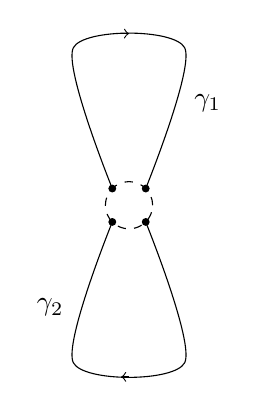
\begin{tikzpicture}
    \draw[dashed] (0,0) circle (.3);

    \fill (.3*.707, .3*.707) circle (.05)
          (.3*.707, -.3*.707) circle (.05)
          (-.3*.707, .3*.707) circle (.05)
          (-.3*.707, -.3*.707) circle (.05);
          %(0,2.18) circle (.05)
          %(0,-2.18) circle (.05);

    \draw[->] plot coordinates {(-.1,2.18) (0,2.18)};
    \draw[smooth] plot coordinates {(-.3*.707,.3*.707) (-.707, 2) (.707, 2) (.3*.707,.3*.707)};

    \draw[smooth] plot coordinates {(-.3*.707,-.3*.707) (-.707, -2) (.707, -2) (.3*.707, -.3*.707)};
    \draw[<-] plot coordinates {(-.1,-2.18) (0,-2.18)};

    \draw (1,1.3) circle (0) node {$\gamma_1$};
    \draw (-1,-1.3) circle (0) node {$\gamma_2$};
\end{tikzpicture}